\documentclass[conference]{IEEEtran}

\usepackage[T1]{fontenc}
\usepackage[latin9]{inputenc}
\usepackage{amsmath}
\usepackage{amssymb}
\usepackage{subscript}
\usepackage{color}
\usepackage[labelfont=bf]{caption}
\usepackage{pgf-pie}
\usepackage{enumitem}




\makeatletter

%%%%%%%%%%%%%%%%%%%%%%%%%%%%%% LyX specific LaTeX commands.
%% Because html converters don't know tabularnewline
\providecommand{\tabularnewline}{\\}

\newcommand{\todoc}[2]{{\textcolor{#1} {\textbf{[[#2]]}}}}
\newcommand{\todo}[1]{{\todoc{red}{\textbf{[[#1]]}}}}

\newcommand{\todored}[1]{\todoc{red}  {\textbf{[[#1]]}}}
\newcommand{\todoblue}[1]{\todoc{blue}{\textbf{[[#1]]}}}
\newcommand{\todogreen}[1]{\todoc{green}{\textbf{[[#1]]}}}
\newcommand{\todoorange}[1]{\todoc{DarkOrange}{\textbf{[[#1]]}}}
%% Additional todo commands:
\newcommand{\TODO}[1]{\todored{#1}}
\newcommand{\sung}[1]{\todored{Sung: #1}}
\newcommand{\shiv}[1]{\todoblue{Shiv: #1}}
\newcommand{\jim}[1]{\todoblue{Jim: #1}}

\newcommand{\zhongpeng}[2]{\todoblue{ZhongPeng: #2}}
\newcommand{\code}[1]{\smalltt{#1}}

%\newcommand{\pparagraph}{\paragraph {\indent}}

%%%%%%%%%%%%%%%%%%%%%%%%%%%%%% User specified LaTeX commands.
\@ifundefined{definecolor}{\usepackage{color}}{}

\usepackage{multirow}
\usepackage{algorithm}
\usepackage{threeparttable}
\usepackage{epsfig}
\usepackage{amsfonts}
\usepackage{cite}
\usepackage{array}


%\usepackage{babel}

\makeatother

\begin{document}

\title{Effective Bug Fix Suggestions}

\author{\IEEEauthorblockN{Shivkumar Shivaji \IEEEauthorrefmark{1},
Zhongpeng Lin \IEEEauthorrefmark{1}, E. James Whitehead, Jr. \IEEEauthorrefmark{1},
Ram Akella \IEEEauthorrefmark{1}, 
Sunghun Kim \IEEEauthorrefmark{2}}
\IEEEauthorblockA{ \IEEEauthorrefmark{1}School of Engineering\\
University of California Santa Cruz, \\
Santa Cruz, CA, USA\\
Email: \{shiv, ejw, ram\}@soe.ucsc.edu
}
\IEEEauthorblockA{ \IEEEauthorrefmark{2}Department of Computer Science\\
Hong Kong University of Science and Technology\\
Hong Kong\\
Email: hunkim@cse.ust.hk
}}
% 
% \authorinfo{Shivkumar Shivaji \and Zhongpeng Lin \and E. James Whitehead Jr. \and Ram Akella }
% 		 {University of California Santa Cruz}
% 		 {{shiv, zlin, ejw, ram}@soe.ucsc.edu}
% \authorinfo{Sunghun Kim}
% 		 {Hong Kong University of Science and Technology}
% 		 {hunkim@cse.ust.hk}
		
\maketitle

\begin{abstract}

There are times when bug fixes are truly one-of-a-kind code solutions to repairing the functionality of a software project. However, it is frequently the case that bug fixes exhibit regularity in the method calls, variables, and programming language keywords used. This paper first presents a technique for learning the conditional probability of a programming language token appearing in a bug fix change given the appearance of a token in a software change predicted to be buggy. The collection of these conditional probabilities is computed by the Bug Fix matrix.

A technique called Fix Suggester uses the Bug Fix matrix to predict those tokens most likely to appear in a bug fix for a given buggy software change. An analysis of the predictive performance of Fix Suggester is performed on four open source projects. Predicted bug fix tokens appear useful in providing developers with clues about how to make bug fix changes.

\end{abstract}
% \category{D.2.5} {Testing and Debugging}{Debugging aids}
% \category{D.4.8} {Performance}{Modeling and prediction}

\begin{IEEEkeywords}
	Modeling and prediction, Debugging aids
\end{IEEEkeywords}


\section{Introduction}

\begin{table*}[t]
\caption[top]{Example bug and fix changes for Argouml Issue \#1104}

\begin{center}
%\begin{tabular}{|l|l|}
\begin{tabular}{lll}

\hline
Bug-introducing Revision 754        & Fix Revision 965                  \\ \hline
\ldots                       & \ldots                      \\
1: public void insertUpdate( final DocumentEvent p1)\{ & 1: public void insertUpdate( final DocumentEvent p1)\{ \\
2: \_textChanged=(\_oldPropertyValue != null) \&\& & 2: if (\_viaUserInput) \{ \\
3: !getText().equals(\_oldPropertyValue); & 3: \_textChanged= \textbf{ !getText().equals(\_oldPropertyValue); \} }\\
4: handleEvent(); & 4: handleEvent(); \\
5: \} & 5: \}  \\
\ldots                       & \ldots                      \\ \hline

\end{tabular}
\end{center}

\label{table:argouml_code_example}
\end{table*}

Recent years have witnessed an increase of research interest in bug prediction techniques. A promising type of bug prediction algorithm uses machine learning techniques to predict whether a specific project change, as committed to a configuration management system, is a buggy change. Examples of such techniques can be found in \cite{Kim2007p58, shivaji2009reducing, aversano2007lbi, Hata2008} with the best such techniques achieving high precision (changes predicted as buggy are very likely to be buggy), and reasonable recall (while not all buggy changes can be detected, a usefully large fraction are).

A notable challenge with such bug prediction algorithms is the nature of their output. They provide just a simple ``buggy/clean'' prediction for each change made to a project. That is, they take a change that a developer has just committed, presumably with some confidence in its correctness, and then simply state that the change is buggy, with no further feedback. We suspect that such bug prediction output might be more acceptable to developers should they additionally receive useful suggestions on how to go about fixing the predicted bug.

Ideally a developer would like reasons for a code change being predicted as buggy along with suggestions on how to fix a bug. This paper proposes a solution that uses project history to statistically predict
the content of future bug fixes to a buggy code change. Predicting the full content of a
bug fix in verbatim is an extremely hard problem.  The proposed solution
instead predicts and suggests unordered programming language tokens
that are likely to appear in a future bug fix.

A developer can use fix suggestions when constructing a bug fix. Table \ref{table:argouml_code_example} contains a buggy change and a part of its fix from the Argouml project. The bug, issue \#1104, was reported as ``UMLTextField generates propertyset events when handling one''. The propertyset() method on a UMLTextField calls update(). Update() in turn sets a property, calling propertyset() again. An event storm results.

The fix suggestion approach in this paper, called ``Fix Suggester'', predicted that the first code change is indeed buggy. It also predicted that the bug fix will involve the programming tokens ``!getText().equals(.)'', ``getText().equals()'', and ``UMLTextProperty.setProperty(,,)''. The actual bug fix was rather lengthy but did modify ``!getText().equals'' as indicated in line 3 of the bug fix. A conditional added in a different intermediate commit is reflected in line 2 of the bug fix.

The goal of fix suggestions is to provide programming language tokens that are likely to be present in an actual bug fix. Correctly predicting a fair amount of tokens present in the actual bug fix indicates a high level of precision. On the other hand, even if Fix Suggester's predicted tokens are in the actual fix, it might have missed many more tokens in the fix. It is desirable to have good coverage of tokens in the bug fix. This is also known as the predication recall of Fix Suggester. Having a reasonable degree of precision and recall will enable the system to be useful in practice.


We envisage a future where engineers have bug prediction and fix suggestions built in to their development environment.
They will receive a prediction on an impending code change followed by a list of potential
bug fix suggestions.
% The presented approach starts with code changes from project history.
% It learns from changes marked as bug inducing and fixes from project
% history.
%These are computed using the SZZ algorithm.
% It requires as
% input the set of fix changes for a particular buggy code change.
% Reasons
% for the bug are then computed.
%These are typically keywords involved in a code change.
% Regions of the code change likely to be addressed by a bug fix are separately
% computed using the bug fix matrix, section ref. These are distinct from the reasons for a bug.

The fix prediction process learns from code changes extracted from a project's source control history. After sufficient
training from history, a bug prediction classifier and a Bug Fix Matrix are built. The matrix contains a map of term frequencies from tokens in buggy changes to tokens in fix changes. Fix Suggestions for a new buggy code change are then predicted by jointly using the bug prediction classifier and the Fix Matrix.

This paper explores the following research questions.

\textit{RQ1. What is the prediction accuracy of the Fix Suggester on varying points of project history?}

RQ1 addresses the accuracy and utility of the Fix Suggester in practice. Fix content is predicted at varying points of project history using
only the information before that point in history. A classifier
and a Bug Fix Matrix are used in combination to train and predict fix tokens that occur. Section
\ref{FixPred} details the methods used for predicting
bug fix content. Section \ref{FixContentPredictionResults} talks
about the results obtained from the approach. Validation is performed by comparing against tokens present in actual bug fixes.

Once fix suggestions are shown to be quite usable, the next logical question is how effective are fix suggestions in practice.
The next two research questions address the utility of the Fix Suggester to engineers.

\textit{RQ2. When engineers inspect the bug fix change log, do they find that the suggested keywords are relevant to the actual bug fix?}

\textit{RQ3. Does reviewing the Fix Suggester's keywords influence the investigation for the bug fix?}

The primary contributions of this paper is a novel method to predicting bug fix content using inputs from a Bug Fix matrix and a classifier. 

In the remainder of the paper, we start by introducing the corpus of projects, performance metrics and research questions. Next, the approaches proposed in the paper are covered in section \ref{Approaches}. This section starts by describing the overall workflow, moves
on to the bug prediction approach, followed by the fix suggestion approach.

The stage is now set to discuss results. The paper starts by detailing answers to the research questions
described above.
The paper ends with an overview of related work (Section \ref{RelatedWork}),
threats to validity (Section \ref{ThreatsToValidity}), and the conclusion.

\section{Experimental Design}
\subsection{Corpus}
\label{Corpus}
The corpus of projects used in this paper
consist of ArgoUML%
\footnote{http://argouml.tigris.org/%
}, Eclipse JDT Core%
\footnote{http://www.eclipse.org/jdt/core/index.php%
}, jEdit%
\footnote{http://www.jedit.org/%
}, and Apache Lucene%
\footnote{http://lucene.apache.org/%
}. Instead of dealing with a small sample of revisions, we have chosen
to go over long revision periods in each of these projects. The rationale
was that large project histories better resemble real world practices.
Table \ref{tab:projects} contains details about the projects we analyzed.


\begin{table*}
\caption{Projects}

\begin{center}
\label{tab:projects}
\setlength{\extrarowheight}{2pt}

\begin{tabular}{cccccp{2.3cm}}
\hline 
\textbf{Name}  & \textbf{Revision}  & \textbf{\# of Total}& \textbf{Buggy}& \textbf{Fix}& \textbf{Neutral}\tabularnewline
& \textbf{Period}  &\textbf{Commits} & \textbf{Commits}&\textbf{Commits}&\textbf{Commits}\tabularnewline

\hline 
ArgoUML  & 01/26/1998 - 06/13/2011  & 17452 & 1516 & 536& 15400\tabularnewline
\hline 
Eclipse JDT Core  & 06/05/2001 - 04/20/2011  & 17904 & 6640 & 4232& 7032\tabularnewline
\hline 
jEdit  & 09/02/2001 - 07/02/2010  & 6050& 3141& 2046& 863\tabularnewline
\hline 
Apache Lucene  & 09/11/2001 - 06/23/2011  & 5966& 1923& 1464& 2579\tabularnewline
\hline
Average &N/A&11843&3305&2069.5&6468.5\tabularnewline
\hline
Average Percentage& N/A&100 &27.9&17.5&54.6\tabularnewline
\hline
\end{tabular}
\end{center}


\end{table*}

\subsection{Performance Metrics}
\label{section:PerformanceMetrics}


\par We now define common performance metrics used to evaluate classifiers:
Accuracy, Precision, Recall, and F-Measure.

There are four possible outcomes while using a classifier:
\begin{itemize}
  \item $tp$, true positive. The classifier correctly predicts a positive outcome.
  \item $tn$, true negative. The classifier correctly predicts a negative outcome.
  \item $fp$, false positive. The classifier incorrectly predicts a positive outcome.
  \item $fn$, false negative. The classifier incorrectly predicts a negative outcome.
\end{itemize}

In this paper, classification was used both for change classification and fix prediction. While the focus is on fix suggestion, 
it is useful to express classification outcomes for both contexts. A classifier's prediction is typically binary. When change classification is performed, a code change is classified as buggy or clean.

During change classification, a true positive is correctly predicting a code change as buggy. A true negative is correctly predicting a clean change as clean. 
A false positive is when a clean change is predicted as buggy. Finally, a false negative is when a classifier predicts a code change to be clean when it is actually buggy. 

The meaning of these outcomes differs for fix prediction. During this process, a prediction is made on every element of a promising group of code tokens. Each token is classified as present or absent in eventual bug fix. A true positive means that a predicted fix code token is present in the actual bug fix. A true negative means that a token not predicted to be in the fix was absent in the actual fix. 
A false positive indicates that a token predicted to be in the fix is not in the actual fix. Finally, a false negative indicates that a token not predicted to be in the fix is present in the actual fix.

%
%\par 
%Correcting predicting a token in a bug fix, $tp$ (true positive) \\ 
%Missing a token that occurs in a bug fix, $fn$ (false negative) \\
%Correctly predicting that a token will not occur in a bug fix, $tn$
%(true negative) \\
%Predicting that a token will occur in a bug fix when in reality it does not,
%$fp$ (false positive)

\par With a good set of training data, it is possible to compute the number of true positives $n_{tp}$, true negatives $n_{tn}$, false positives $n_{fp}$, and false negatives $n_{fn}$.
 $$Accuracy = \dfrac{n_{tp} + n_{tn}}{n_{tp} + n_{tn} + n_{fp} + n_{fn}}$$
    Accuracy is the number of correct predictions over
 the total number of predictions. Bug prediction typically deals with more clean
 changes than buggy changes. Using this measure could yield a high
 value if clean changes are being better predicted than buggy
 changes. During fix content prediction, accuracy does not reveal the disparity between false positives and false negatives. Overall, the accuracy figure is often less relevant than precision and recall. 
 
$$Precision, P = \dfrac{n_{tp}}{n_{tp} + n_{fp}}$$
   For buggy change prediction, its the number of code changes which are actually buggy when predicted to be buggy. For fix content prediction,
   this represents the number of correct predictions over the total number of tokens predicted to be in the fix.
   
$$Recall, R = \dfrac{n_{tp}}{n_{tp} + n_{fn}}$$

  Also known as the true positive rate, this represents the number of correct bug classifications over the total number
  of changes that were actually bugs. For fix content prediction, its the likelihood that a token in an actual bug fix was predicted by the classifier.
  
$$F-measure = \dfrac{2 *P* R} {P+R}$$

   This is a composite measure of buggy change precision and
recall, more precisely, it it the harmonic mean of precision and
recall. Since precision can often be improved at the expense of recall
(and vice-versa), F-measure is a good measure of the overall precision/recall
performance of a classifier, since it incorporates both values.
For this reason, we emphasize this metric in our analysis of 
classifier performance in this paper. 

An extreme example is when the Fix Suggester predicts no tokens for a code change. This results in a precision of 100\% and a recall of 0\%. Predicting all tokens in a vocabulary leads to 100\% recall at huge cost to precision. Presenting the F-measure allows one to better understand the precision recall tradeoff. Accordingly, Figure \ref{Figure:FixSuggesterResults} relays fix content prediction F-measure throughout project history for all corpus projects. Several data/text mining papers have compared performance on classifiers using F-measure including \cite{Anagnostopoulos2006p1049} and \cite{larsen1999fae}.

In this paper, the precision, recall, F-measure metrics refer to the class of code tokens which are predicted to be part of a fix. For bug prediction, these metrics refer to changes which are predicted to be buggy. One can also use precision and recall to refer to changes which are predicted to be clean or to predict tokens which are not part of a future fix. For the sake of simplicity, this paper refers to precision and recall in the straightforward context of predicting a change to be buggy and predicting fix tokens of a future bug fix.

The next section describes the change classification and the Fix Suggester in detail. 

\section{Approaches}
\label{Approaches} 

\begin{figure}[t]
\begin{center}
 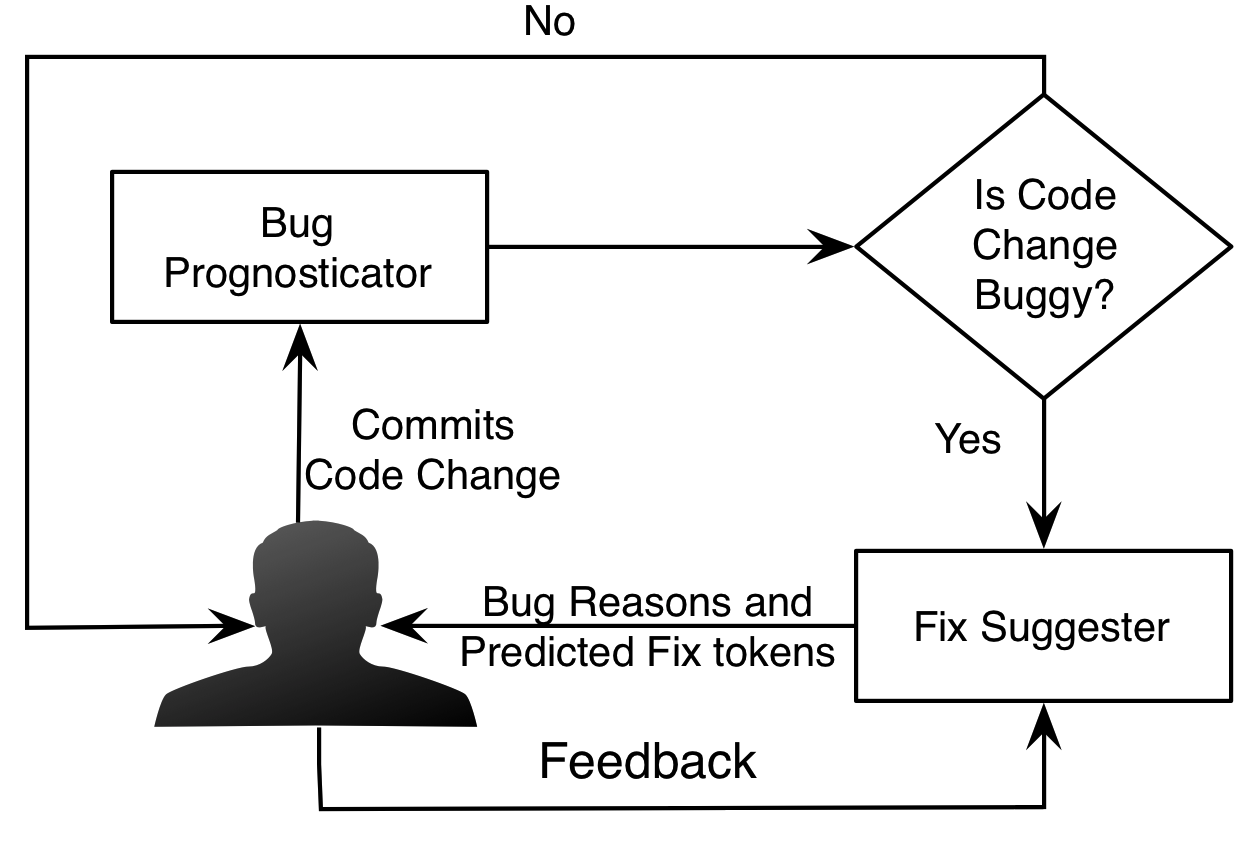
\includegraphics[scale=0.75]{pictures/HumanWorkflow.png}
\end{center}
\caption{Developer Interaction Workflow}
\label{workflow}
\end{figure}



In this section, we distill the approaches used in the paper, starting with the code change classifier followed by the Fix Suggester. An overview of the developer interaction workflow is depicted in Figure~\ref{workflow}.
The steps of the process are:
\begin{enumerate}
\item A code change is submitted.
\item A prediction is made on whether the entire change is buggy or clean using change
classification~\cite{Kim2007p58, shivaji2009reducing}. Change classification is explained in Section~\ref{ChangeClassification}.
\item If the code change is predicted to be buggy, suggest a partial code fix.
The predicted fix tokens are presented to the user. The Fix content prediction algorithm is described in
Section~\ref{FixPred}.

\end{enumerate}

The next subsections describe these steps in detail. 

\subsection{Change Classification}
\label{ChangeClassification}

\begin{figure}[t]
\begin{center}
 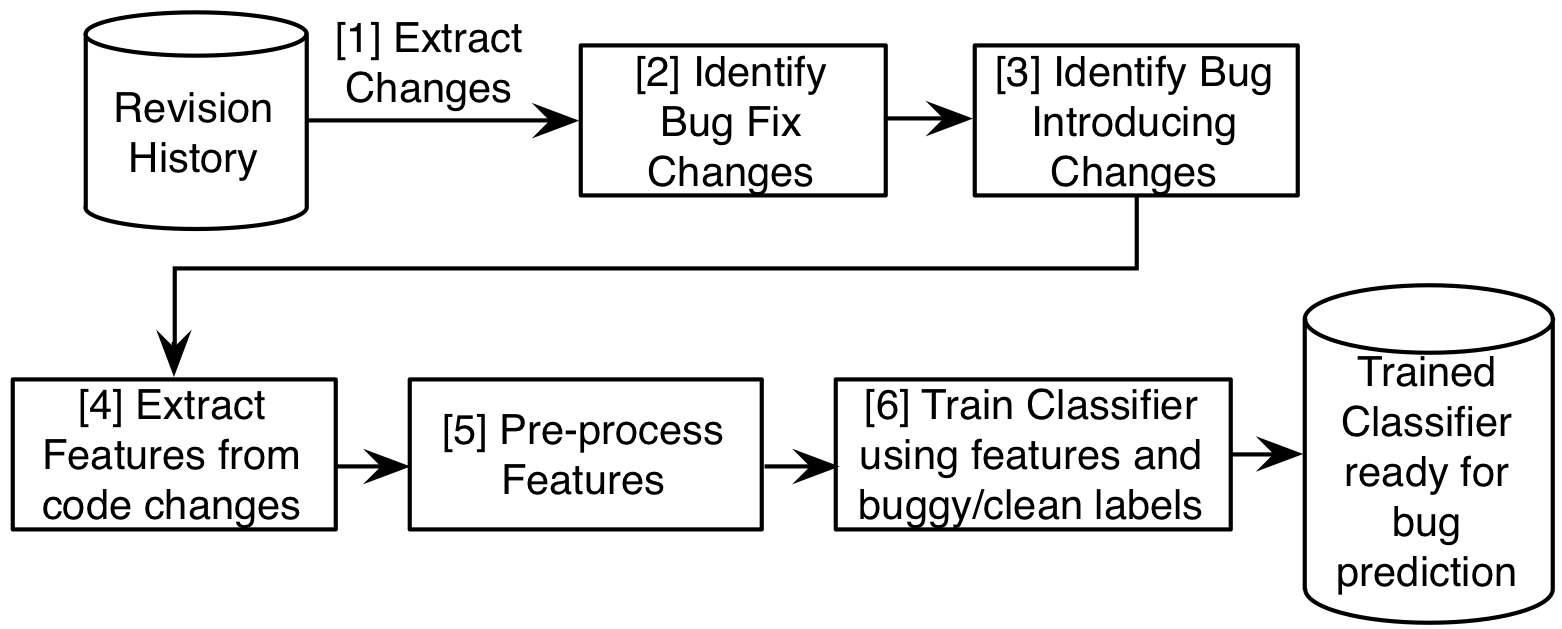
\includegraphics[scale=0.65]{pictures/BugPred.png}
\end{center}
\caption{Change Classification Setup}
\label{bugpredWorkflow}
\end{figure}

Change classification is an algorithm used to label and predict code changes as buggy or clean. 
The key steps of the algorithm are briefly described in this section.
For a detailed
description of the algorithm, refer to~\cite{Kim2007p58, shivaji2009reducing}.

The change classification process is distilled in Figure \ref{bugpredWorkflow}. The primary steps involved in performing change classification 
%on a single project 
are outlined as follows: 
\begin{enumerate}
\item File level changes are extracted from the revision history of a project,
as stored in its SCM repository. 
\item The bug fix changes for each file are identified by examining keywords
in SCM change log messages or cross-referencing with a bug tracking
database such as Bugzilla. 
\item Bug-introducing and clean changes at the file delta level are identified
by tracing backward in revision history from bug fix changes~\cite{Sliwerski2005} as described in Section~\ref{FindingBuggyCleanChanges}.
\item Features are extracted from all changes, both buggy and clean. Features
can include all terms in the complete source code, the lines modified
in each change (delta), AST metrics, and change
metadata such as author and change time as listed in Section~\ref{FeatureExtraction}
\item The extracted features are from many different sources and have differing value ranges. The various features are all transformed to a [0,1] scale using different techniques during the feature pre-processing step.
\item Historical code change data with features and labels (buggy or clean) can be used to train a classifier. The classifier can then
predict if future changes are buggy or clean.
\end{enumerate}

\subsubsection{Finding Buggy and Clean Changes}
\label{FindingBuggyCleanChanges} In order to find bug-introducing
changes, bug fixes must first be identified by mining change log messages.
We use two approaches: searching for keywords in log messages such
as ``Fixed\textquotedbl{}, ``Buggy\textquotedbl{} {[}4{]}, or other
keywords likely to appear in a bug fix and searching for references
to bug reports like ``\#42233\textquotedbl{}. This allows us to identify
whether an entire code change transaction contains a bug fix. If it
does, we then need to identify the specific file change that introduced
the bug. The bug-introducing change identification algorithm proposed
by Sliwerski, Zimmermann, and Zeller (SZZ algorithm)~\cite{Sliwerski2005}
is used in the current paper. After identifying bug fixes, SZZ uses
a difference tool to
determine what changed in the bug fixes. SZZ tracks down the origins of the modified hunks in the bug fix. The discovered origins are labeled as buggy changes.

\subsubsection{Feature Extraction}
\label{FeatureExtraction} A commit to a source code repository involves
two source code revisions (an old revision and a new revision) and
a change delta that records the added code (added delta) and deleted
code (deleted delta) between the two revisions. A commit has associated
meta-data, including the change log, author, and commit date. Every
term in the source code, change delta, and change log texts is used
as a feature. Eight features are gathered from commit meta-data: author,
commit hour, commit day, cumulative change count, cumulative bug count,
length of change log, changed LOC (added delta LOC and deleted delta
LOC), and new revision source code LOC.

To generate features from source code, we use a modified version of
the bag-of-words approach (BOW), called BOW+, that extracts operators
in addition to all terms extracted by BOW~\cite{Kim2007p58}, since
we believe operators such as !=, ++, and \&\& are important terms
in source code. We perform BOW+ extraction on added delta, deleted
delta, and new revision source code.

For this paper, select AST features were added to the typical change
classification algorithm. The change distilling algorithm proposed by
Fluri et al.~\cite{Fluri2007} was used to extract the difference between abstract
syntax trees (ASTs) built from the old and new revisions for each commit. The change distilling algorithm categorizes changes
of ASTs into 48 types, according to the taxonomy defined by their
previous work~\cite{Fluri2006}. The number of occurrences
for each change type was used as a feature.

A vocabulary of features was built from the first 500 revisions for each project in the corpus. 
This vocabulary of features is used by buggy, fix, and neutral revisions. Any new token brought in after revision 500 will not be used for bug prediction or Fix Suggestions. 
This was done In order to ensure that the Fix Suggester can be used after revision 500 without adding new rows or columns to the Fix Matrix.

Each of these features can have largely differing sets of values. With differing
value ranges, it is challenging to use the data. The next section
deals with pre-processing features so that their value ranges are
comparable.

\subsubsection{Feature Pre-processing}
This section explores the different kinds of features present in the data sets and techniques to align data for efficient analysis of code changes.

Keyword features
can potentially have a large range of values if one uses their frequency of occurrence in code changes. 
There is a choice on how to interpret this feature, one can either
record the presence of a keyword feature or record the number
of times the keyword appears in a code change. 

For example, if a variable maxParameters is present anywhere in the
project, a binary interpretation of this feature records this
variable as being present or absent, respectively 1 or 0 for a code change. A count interpretation would instead
record the number of times it appears for a particular code change. It
was observed that large values when using count tended to skew bug fix
prediction. Employing a binary interpretation additionally allows
one to simplify fix prediction to the presence of a keyword in a code change, instead of the number of times a keyword will appear in a fix.
Thus, a binary interpretation was used for keyword features. This limits
the range of values to 0 and 1 for keyword features.

Numeric meta-data features such as LOC, cumulative change count, cumulative
bug count, length of a change log can have unpredictable ranges as
well. These were numerically scaled to the [0, 1] range using rudimentary numerical transformations~\cite{saunders1998support}. 

AST features presented a different problem. While AST feature values
do have a large range of values, the range is much smaller than keyword
features. These were scaled to the [0,1] range, similar to numeric meta-data
features.

Categorical features such as author name, commit hour (0-23), and
commit day (1-7) were not numerically scaled. One cannot conclude
that a code change committed at 2pm is twice as important as a 1pm
code change. These features were thus converted to binary terms. For example
if commit day is 2, commit\_day\_is\_2 would be 1 and commit\_day\_is\_1,
commit\_day\_is\_3, .., commit\_day\_is\_7 will all have zero values.
The benefit of using binary values for these features is removing
any numerical bias during analysis. 

The data is now transformed to the [0,1] range.

Once the features are extracted, processed, and training is performed on sufficient revisions, a new code change can be classified as buggy or clean. 
The next section introduces an approach to predict bug fix content for a predicted buggy change.

%\sung{It seems like this is our new contribution. Why it is in the background?}

\subsection{Fix Suggester}
\label{FixPred} 


The goal of the Fix Suggester is to accurately predict code tokens of a fix to the current buggy change. Typically predicting code tokens of a fix means predicting
them in the order that they would appear in a fix.
However, predicting the code tokens of a fix in verbatim is a very difficult problem. Fix Suggester, in this paper, instead
predicts unordered programming language tokens of a future bug fix to a presented buggy code change.
In this paper, contents of a bug fix are synonymous with the terms of a bug fix.
These are in turn synonymous with fix suggestions.

We denote a buggy revision as B\textsubscript{n}. The corresponding fix to this revision F\textsubscript{n} occurs later in time.

%Fix content prediction aims to predict tokens of F\textsubscript{n} given revision B\textsubscript{n} and all prior revisions.

The inputs to fix prediction are:
\begin{itemize}
\item A code change predicted to be buggy, revision B\textsubscript{n}.
\item All previous revisions annotated as buggy, a bug fix, or neither.

\end{itemize}

The output is a set of code tokens that are likely to be present in revision
F\textsubscript{n}. A good fix prediction will have a high intersection among
predicted tokens and the actual tokens of F\textsubscript{n}. 

A function that links tokens of B\textsubscript{n} to the tokens of F\textsubscript{n} is desirable for predicting fix content accurately.
As most of the features extracted are keyword features, a link between buggy and fix keywords is helpful. This work focuses on
statistical approaches to link buggy and fix tokens. The next section
details the Bug Fix Matrix, an approach that predicts bug fix content using the modified data.

\begin{table}
\caption{Bug Fix Matrix Example}

\centering
\begin{tabular}{cccc}
\hline
 & File & File.open() & File.close()\tabularnewline
\hline
\hline 
File & 2 & 0 & 1\tabularnewline
\hline 
File.open() & 0 & 0 & 1\tabularnewline
\hline 
File.close() & 1 & 0 & 0\tabularnewline
\hline 
\end{tabular}

\label{fig:exampleFixMatrix}
\end{table}


\subsubsection{Bug Fix Matrix}

The Bug Fix matrix generates a set of term frequencies among past buggy and fix tokens. It can then be used to predict tokens of a new buggy revision.

Suppose we had the following three keywords in
a few code changes: File, File.open(), File.close(). An example fix
matrix is depicted in Table~\ref{fig:exampleFixMatrix}. The matrix indicates that if there is a \textquotedbl{}File\textquotedbl{}
keyword in the bug, amongst all the bug fixes, ``File.close()''
was present once in the bug fix. The bug fix in 2 cases added/modified
``File'' and in one case added a ``File.close'' when ``File''
is in the bug inducing change. When ``File.open()'' was present
in the bug, the bug fix added a ``File.close()''. The matrix reflects
a bug when a developer opens a file but forgets to close it. The bug
fix calls File.close().

The Fix matrix generates a buggy to fix frequency map between all terms of the vocabulary generated in section \ref{FeatureExtraction}.
Feature i represents a particular token of the vocabulary. The left column of the matrix represents a token from a buggy code change.
Each row of the matrix indicates the number of times a token shows up on the bug fix given presence of a token in the buggy change. For example,
 ${M_{i,j}}$ = 1 means that for all buggy changes where token i was present, in only one of them token j was present in the bug fix. The Fix matrix
 can mention how often the same token i occurred in both the buggy change and the fix via ${M_{i,i}}$. In order to make sense out of the Fix matrix's output, all term frequencies were scaled to the [0,1] range. This avoids bias against frequently occurring tokens and simplifies the fix prediction process.


\begin{figure}[t]

\begin{center}
 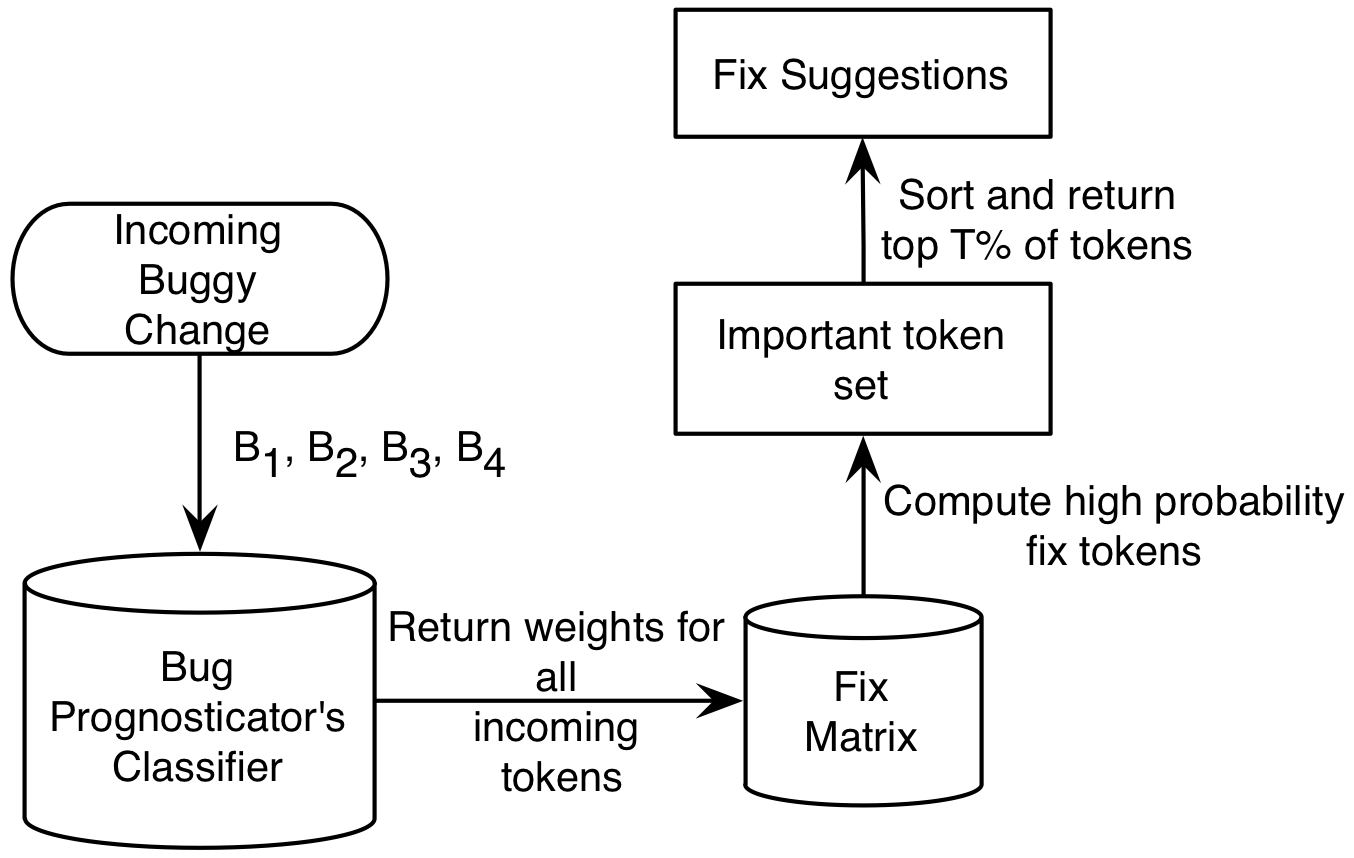
\includegraphics[scale=0.75]{pictures/FixSuggester.png}

\end{center}
\caption{Fix Suggester}
\label{Fig:FixSuggester}

\end{figure}

The Bug Fix Matrix can be used to predict fix content for an incoming buggy change. The Fix  Suggester's algorithm is illustrated in Figure \ref{Fig:FixSuggester} and detailed in Algorithm \ref{FixSuggesterAlgorithm}.
\begin{algorithm}
\caption{Fix Content Prediction Algorithm}

\begin{enumerate}
\item A potentially buggy code change is given as input.
%\item Create a fix matrix on the training set of bug inducing changes and their respective fixes up to this point.
%\item Calculate the probability of occurrence in the bug fix for every token in the vocabulary.
\item For a new bug inducing code change, use the bug prediction classifier to return weights for all incoming buggy tokens.
\item Multiply the term frequency of each predicted fix token by the classifier weight for the source buggy feature if it is present.
\item Store all candidate fix tokens in imp\_set.
\item Sort the list of features in imp\_set by their conditional probability.
\item Return top T percent of high probability fix tokens from imp\_set.
\end{enumerate}
\label{FixSuggesterAlgorithm}
\end{algorithm}

In step 2, the fix matrix entries are adjusted using information from the code change classifier.
The SVM algorithm assigns a weight to each feature, with a higher weight indicating that this feature is more useful in separating buggy changes from clean changes.
We assume that these same features are also more useful for predicting which keywords will appear in bug fixes as well, and hence we wish to emphasize these keywords in the fix matrix.
To accomplish this, we multiply each matrix entry associated with a token by its SVM weight (as found in the SVM primal weight vector w in the Liblinear implementation [12]).

For each buggy token entry on the left side of the matrix, all tokens in the columns followed by their weight are returned to imp\_set. Once the conditional probability of being a fix token is computed for all tokens in the vocabulary, a good cutoff is needed for the final step of extracting high probability fix tokens from imp\_set. 
The top 10 percent of tokens with the highest conditional probabilities were returned. Fix Suggester's results are summarized in section \ref{FixContentPredictionResults}.

An important practical issue with the Fix Matrix is the huge size it can encompass. Even using data from the first 500 revisions, the fix matrix vocabulary can still consist of about 50 thousand features. Having a 50 thousand by 50 thousand matrix can contain 2.5 billion
entries. In order to make the algorithm perform well for this paper, only the top 10\% of tokens returns by the classifier were entered into the Fix Matrix. This is a radical compromise to simplify the problem. In order to increase recall at the cost of precision, it might
be useful to include more features and investigate scalable solutions for large matrices.

A lesser practical issue is before predicting a bug fix for a buggy code change, one may not know a priori if a particular code change is buggy to start with.
The SZZ algorithm for example, traces backward from a bug fix to a buggy change.
Not knowing if a change is buggy until a bug fix is performed would mean that fix content prediction itself could be less useful in practice.

However, the benefit of using a classifier driven approach is one can leverage previous work to make a buggy/clean prediction on a code change and return fix content
 only on those code changes which the classifier thinks are buggy.
The code change classifier performed well on all corpus projects, when training on a portion of past project history to predict if future code changes are buggy or clean. 
A separate classifier was used for each project.
It is possible to use an entirely different bug prediction algorithm to predict if a code change is buggy before applying fix prediction.

The next section details results from the Fix Suggester.

\section{Results}
\label{Results}
\subsection{Fix Suggester}
\label{FixContentPredictionResults}

\begin{figure}[t]
\begin{center}
 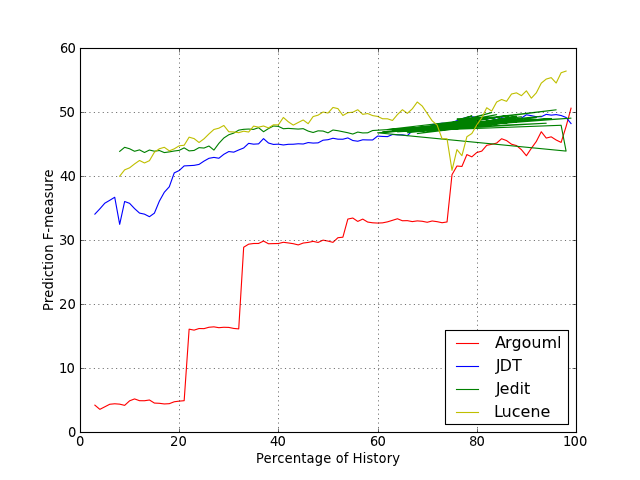
\includegraphics[scale=0.45]{pictures/rq1.png}
\end{center}
\caption{Fix Suggester F-measure on Project History}
\label{Figure:FixSuggesterResults}
\end{figure}



\begin{table}\centering
\caption{Average Fix Content Prediction rate per project from Project History}
\label{tab:AvgFeedback}
\begin{tabular}{cccc}
\hline
Project &  Precision &  Recall &  F-measure\\ 
\hline
Argouml &  39.67 &  21.80 &  27.80\\ 
\hline
Eclipse JDT &  45.26 &  43.81 &  44.47\\ 
\hline
jEdit &  50.85 &  44.62 &  46.89\\ 
\hline
Lucene &  51.93 &  45.18 &  48.28\\ 
\hline
Average &  46.93 &  38.85 &  41.86\\ 
\hline
\end{tabular}

\end{table}

The Fix Suggester was evaluated by training on p\% of project history and testing on (100-p)\% of project histories for p ranging from about 5 precent to 100 percent in 1 percent increments. As the vocabulary was generated using the first 500 revisions, no fix suggestions are presented when there are less than 500 revisions.  In order to grade the efficiency of the Fix Suggester independent of the classifier,
actual bug fixes from test data were compared to the Fix Suggester's fix tokens. In other words, performance of the Fix Suggester was graded on actual future bug fixes by passing in the buggy change and all history prior to the buggy change. Prior history was cleansed to ensure that no information from the future was visible. For example, if a historical code change was labeled buggy due to a future fix, it is modified to reflect a neutral change in order to ensure that predictions do not unfairly use data from the future.

The Fix Suggester is able to achieve an average precision of 46.9\% and
a recall of 38.9\% when averaging the evaluation points over all projects in the corpus. Table \ref{tab:AvgFeedback} contains averaged results by project. Figure \ref{Figure:FixSuggesterResults}
 depicts a historical graph of predicted fix content F-measure vs ratio of project history. Unsurprisingly, fix prediction F-measure improves with more historical project data. It is encouraging that after 500 revisions of project history, fix suggestions are usable for all projects except Argouml.  

Overall, predicting bug fix content is a hard problem. Being able to correctly predict close to 47\% of the actual content of bug fixes while covering almost 39\% of all bug fix tokens is not a bad start. As precision can be improved at the cost of recall, and vice-versa, Figure \ref{Figure:FixSuggesterResults} displays F-measure results instead. If a developer desires more precision at the cost of recall, it is possible to go beyond 47\%. 

These results seem quite promising. In practice, however, having a precision and recall of less than 50\% each might confuse humans when working on a bug fix. In addition, the utility of the proposed keywords should be better understood. The final benefit of a user study focusing on industrial software engineers is evaluating the suitability of corporate adoption of the Fix Suggester. The next section introduces the user study procedure.

\subsection{User Study Procedure}
Fix Suggester results were shown to 19 users for both RQ2 and RQ3. To make analysis convenient, the respondents were asked to complete an online survey showing partial code diff data. SurveyMonkey was used for online delivery of surveys. The majority of participants were industrial software engineers. All participants had some knowledge of Java.

In the case of RQ2, users were asked to indicate if the suggested keywords intersected with the actual bug fix using a Likert scale of 3 options. Participants were shown the Bug Fix change log, parts of the actual bug fix, and the Fix Suggester's keywords.

\begin{description}
	\item[Not Helpful] The predicted keywords did not intersect at all with the actual bug fix.
	\item[Somewhat Helpful] The predicted keywords partially intersect with the actual bug fix.
	\item[Helpful] The predicted keywords intersect with key portions of the bug fix.
\end{description}

A response of ``Not helpful" indicates that despite statistical intersections, the predicted keywords did not actually reflect in the presented extracts of the bug fix. Somewhat helpful connotes clear intersection but not with key portions of the bug fix. Helpful depicts that an intersection exists between the suggestions and key regions of the bug fix.

For RQ3, subjects were shown the bug fix change log comment. They were also shown parts of the actual buggy change. They were asked to form a set of candidate keywords for the bug fix. After viewing the suggested keywords, they were asked if their set of candidate keywords was altered after viewing the fix suggestions. This experiment replicates potential industrial usage of the Fix Suggester. During a typical business day, one can envisage that the content of the bug fix is not yet known, and the Fix Suggester's suggestions have to be evaluated on face value. 

The bug fix change log comments were shown to the users in order to guide their search for the fix. It is hard to isolate potential bug fixes on large set of code changes without any direction. In practice, a bug report, or a customer experience with a bug can be substitutes for the change log comment of the actual bug fix.

The feedback options for RQ3 include

\begin{description}
	\item[Not Helpful] My candidate keyword list was unaffected
	\item[Somewhat Helpful] My candidate keyword list changed somewhat due to the fix suggestions
	\item[Helpful] My candidate keyword list was influenced by the fix suggestions
\end{description}

The option ``Not helpful" in this case means an unaltered candidate keyword list. Somewhat helpful indicates that the candidate keyword list had a moderate change. Helpful means the candidate code list was strongly influenced by the suggestions. Users provided feedback on randomly selected code changes on every project for which fix suggestions were computed.

The next section details results of the qualitative study on the Fix Suggester.

\subsection{Fix Suggester Qualitative Study Results}
\label{FixSuggesterUserStudy}

RQ2 states ``When engineers inspect the bug fix change log, do they find that the suggested keywords are relevant to the actual bug fix?'' 69.5\% of the surveyed engineers found the suggested keywords to be somewhat or quite helpful. 30.5\% of engineers on the other hand found the suggested keywords to not be helpful, they did not see any intersection with the actual bug fix.

RQ3 states ``Does reviewing the Fix Suggester's keywords influence the investigation for the bug fix?'' 67.4\% of engineers found the suggested keywords to be somewhat or quite helpful. 32.6\% of engineers found the suggested keywords to be not helpful, stating that their candidate keyword list was unaffected by the suggestions.

The distribution of utility of the suggestions for RQ2 and RQ3 is respectively shown in figures \ref{Suggester_RQ1_Results} and \ref{Suggester_RQ2_Results}. There was not much deviation from one project to another. It is promising that engineers on average found the Fix Suggester to be somewhat useful for both RQ2 and RQ3.

The general feeling was that the Fix Suggester is quite useful for engineers new to a codebase. Typical co-occurrence patterns of a bug fix were exposed especially for user interface driven projects such as Jedit and Argouml. The patterns are not limited to simple co-occurrence. The Fix Suggester is perhaps a customized filtered version of a co-occurrence driven solution based on fixes applied to similar bugs. These patterns tend to help engineers new to a project. A practical example is the knowledge that getPreferredSize, actionPerformed, setLayout, propertiesChanged are keywords that should be included if bug fix involves changing a UI action in Jedit. Another is that a bug fix on the Lucene index will require changing documents, created, current (document), open (document), and (document) count.

However, there are a few areas for improvement. Firstly, about 30\% of users finding the suggestions ineffective is a clear area to work on for both research questions. The more challenging issue is to sway users who found it to be `Somewhat Helpful'. The following suggestions were based on the verbal feedback provided by the users. 

\begin{description}[leftmargin=\parindent,topsep=0pt,partopsep=3pt,parsep=0pt,itemsep=3pt]
	\item[Large Code Changes]
	The Fix Suggester did not fare well on large code changes for both RQ2 and RQ3. For RQ2, it was especially hard for engineers to look for intersections when code spanned several files. On RQ3, a large keyword list tended to confuse engineers. It might be interesting to adaptively trim the set of recommended keywords on a particular code change. It might also be possible to trim the suggestion list based on how tolerant the user is. Those users finding it not helpful would have benefited from a smaller set of suggestions.
	\item[Reducing Search Time]
	Having extraneous keywords can confuse engineers in practice. For RQ3, this means the search for a bug fix can be derailed by poor/less likely keyword choices. Engineers did not want to waste time on a suggested keyword if it was unlikely to be needed for this fix. A model that tried to minimize wasted time at the cost of missing out a few relevant keywords appealed to them. At first, this appears to be a simple precision/recall tradeoff. However, it is actually a more complex request for lower recall but saving potentially significant human time. Human time can be saved by not including plausible but ineffective keywords. A plausible but incorrect keywords might lure unsuspecting engineers to waste time while considering viabilities for these types of keywords.
	\item[More Detail]
	To sway engineers from viewing the suggestions as somewhat helpful, they seemed to desire more detail on why those keywords need to change in a bug fix. One idea would be to integrate the keyword suggestions with static analysis techniques before presenting them. Static analysis tools like Findbugs often report several detailed violations. Engineers typically ignore the bulk of these violations. If the violations can be filtered by the Fix Suggester, they might be more likely to pay attention given that the Fix Suggester provides statistically relevant bug fix information. Statistics backed by the explanation power of static analysis can possibly be combined to make the suggestions effective.
	\item[User Personalization] 
	About 30\% of users found the suggestions to be not helpful. It might be useful to target suggestions at these users adaptively. If a user was unhappy with a suggestion due to too many keywords, less keywords can be offered the next time. Personalizing the Fix Suggester at the user level will likely increase practical satisfaction.
	
\end{description}

\begin{figure}
	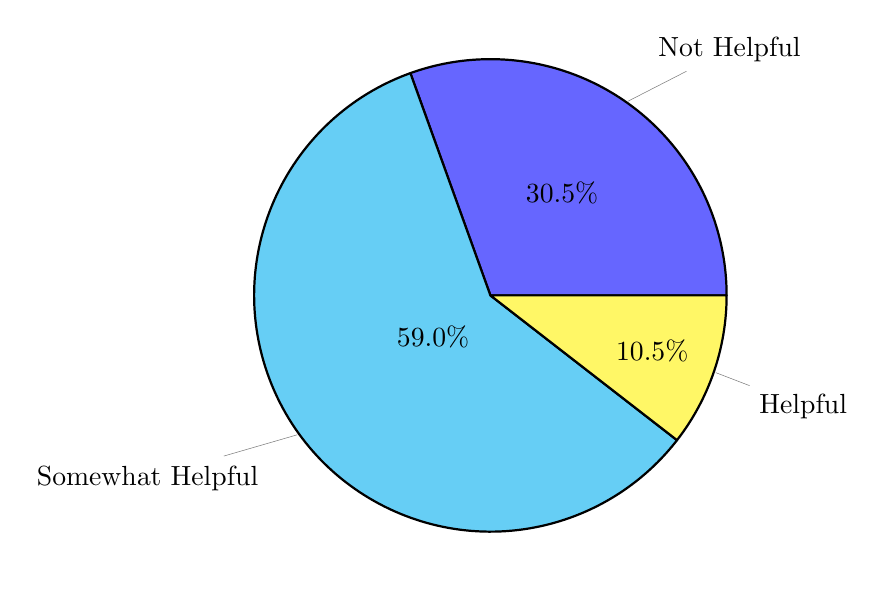
\begin{tikzpicture}
		\pie[text=pin]{30.5/Not Helpful, 59.0/Somewhat Helpful, 10.5/Helpful}		
	\end{tikzpicture}
	\caption{RQ2 Feedback}
	\label{Suggester_RQ1_Results}
\end{figure}

\begin{figure}
	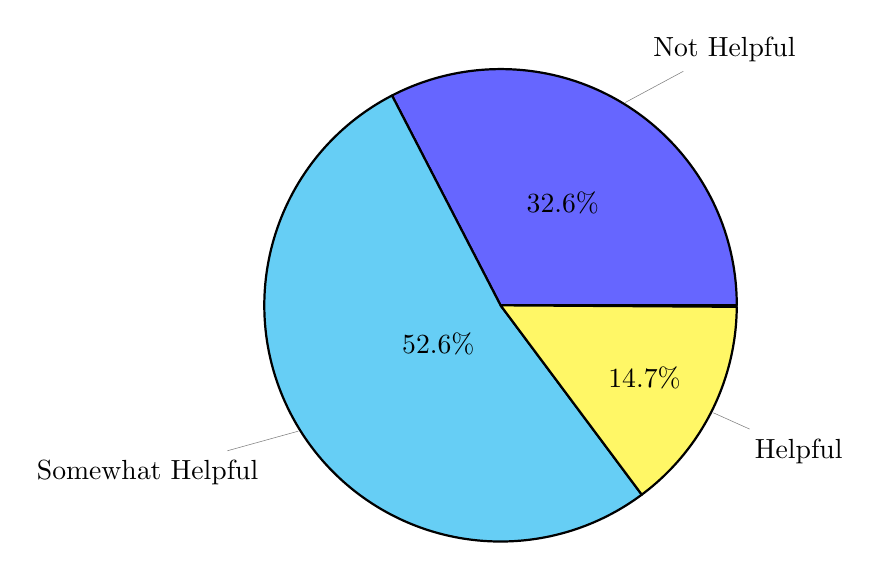
\begin{tikzpicture}
		\pie[text=pin]{32.6/Not Helpful, 52.6/Somewhat Helpful, 14.7/Helpful}		
	\end{tikzpicture}
	\caption{RQ3 Feedback}
	\label{Suggester_RQ2_Results}
\end{figure}

\section{Related Work}
\label{RelatedWork}

\par As this paper touches on a few different techniques, related work can be gathered from one of three phases of figure \ref{workflow}. 


\subsection{Bug Prediction on a Given Software Unit} 
\par Several approaches attempt defect prediction on a given software unit. It is ideal for the software unit to be as small as possible. Prediction on a code change allows an individual change to be targeted for fix content prediction. Aversano et al. \cite{aversano2007lbi} use KNN (K nearest neighbors) to locate faulty modules.  Hata et al. \cite{Hata2008} showed that a technique used for spam filtering of emails can be successfully used on software modules to classify software as buggy or clean. Kim et al. \cite{Kim2007p58} and Shivaji et al. \cite{shivaji2009reducing} perform bug prediction on a code change. The latter technique was used by this paper. D'Ambros et al. \cite{d2011evaluating} perform an extensive comparison of various bug prediction algorithms that operate at the file level.

\par While its preferable for the software unit to be as small as possible in order to optimize the future steps in the process, any of the above methods can be used in place of a code change level bug predictor.

\subsection{Bug Fix Content Prediction}

Suggestions for Bug Fixes can come from different techniques. The most common is via static analysis. Related work not using static analysis is also discussed. 

\subsubsection{Static Analysis Techniques}

Predicting bug fix content is a challenging problem especially when
using statistical techniques. The static analysis community has spent
considerable effort in exploiting language semantics to suggest fixes
to bugs. Popular tools using static analysis for fix suggestions
include Findbugs \cite{ayewah2008using}, PMD \cite{rutar2004comparison}, BLAST \cite{muhlberg2007blast}, FxCop \cite{wagner2008evaluation} amongst many others. There are also approaches from literature which do not yet have downloadable tools available. 

Demsky et al. focused on data structure
inconsistency~\cite{demsky_data_2005,demsky_inference_2006}. Their approach
checks data structure consistency using formal specifications and inserts
run-time monitoring code to avoid inconsistent states. This technique
provides workarounds rather than actual patches since it does not modify source
code directly.

Arcuri et al. introduced an automatic patch generation
technique~\cite{arcuri_automation_2008,arcuri_multi-objective_2008,arcuri_novel_2008}. They used genetic programming. Their evaluation was limited to
small programs such as bubble sort and triangle classification.

The method suggested in this paper
approaches the problem statistically. The general benefits of a statistical
driven approach are:

\begin{itemize}
\item A focus on predicting fix suggestions that will actually be fixed in practice. Wedyan et al.
has analyzed static analysis suggestions and found that less than
3\% of the suggestions are actually fixed in practice \cite{wedyan2009effectiveness}. When interacting
with a few industrial settings, this number was found to be less than
0.5\%. In contrast, the statistical driven approach presented has an average precision greater than 46\% meaning that almost half of the tokens returned by the Fix Suggester will be used in future bug fixes.  
\item Project history is leveraged and automatically tailored for adaptive
prediction of bug fixes relevant to the future code changes of a particular
project. Historical trends can also be exploited. If a particular
type of bug fix was popular at the onset of a project but diminished
in significance soon, statistical fix content prediction will downplay
the importance of that fix pattern.
\end{itemize}

There are benefits to static analysis when compared to statistical
approaches including:

\begin{itemize}

\item The suggested bug fix is an exact solution which can often be proved
in its effectiveness. In contrasts, a statistical approach is a probabilistic
statement on the likely contents of a bug fix.

\item The suggested fix and explanations can be well understood by humans.

\end{itemize}

\subsubsection{Fix Content Prediction Without Static Analysis}
Brun et al \cite{Brun2004p1} use machine learning to detect program properties
which are known to result from errors in code. They rank and classify these properties from user written code. They then warn the user if many
such properties are present.

Nguyen et al. \cite{nguyen2010recurring} recommend bug fixes for a class or method if a fix was applied to a code peer. If a relevant bug fix was applied to a similar class, it is then recommended. Code peers are defined as objects which work in a similar manner when using a graph based representation of object usages.

Kim et al.'s Bugmem provides fix suggestions using past revision history \cite{Kim2006} . Bug and fix pairs are extracted from history. If an impending code change is similar to a previous bug, the prior buggy change and bug fix are displayed, and the developer is warned. This is a useful tool especially for developers who are new to a code base. They can be alerted of mistakes from project history. 

Weimer et al. use genetic learning to suggest a fix based on mutations of the ASTs of the source hunks \cite{Weimer:2009:AFP:1555001.1555051}. If there is a
comprehensive set of unit tests, and a bug was introduced which broke a unit test, this technique can repair that unit test using genetic
learning and mutating AST of the source hunks until all unit tests pass again. The limitation of this technique is the assumption that unit
tests are comprehensive and the fact that the fix suggested may not be optimal or even a feasible one.

Holmes and Murphy proposed an approach to extract structural components from example code and use them to assist coding when developers are working on similar code \cite{holmes2005using}.

The approach presented in this paper is similar to BugMem and Holmes et al. in that suggestions are made for a particular code change. The difference is that the recommended tokens are continuously validated against actual bug fixes. This ensures that the fix recommendations are likely to appear in actual fixes.

In the field of information retrieval, matrices are often used to represent document similarity \cite{rolleke2006general}. While fix content prediction is a different problem, representing bugs and fixes as problem spaces and relating these spaces using a matrix has a high level parallel. The matrix relating buggy changes to fixes modelled a linear relationship in this paper. Future work can extend the concept to capture more complex relationships between buggy and fix changes.


\section{Threats to Validity}
\label{ThreatsToValidity}

\par \textbf{Systems examined might not be representative of typical projects.} \\
Four systems with large histories are examined. In spite of this, it is still possible that we accidentally chose
systems that have better (or worse) than average fix suggestion prediction accuracy. Since we
intentionally chose systems that had some degree of linkage between change tracking
systems and change log text (to determine fix inducing changes), there is a
project selection bias.

\par \textbf{Systems are open source.} \\ The systems examined in this paper use an open source
development methodology, and hence might not be representative of typical development contexts. It
is possible that more deadline pressure, differing personnel turnover patterns, and varied
development processes used in commercial development could lead to different bug fix
patterns.

\par \textbf{Bug fix data is incomplete.} \\ Even though we selected projects that have decent change logs,
we still are only able to extract a subset of the total number of bugs (typically only 40\%-
60\% of those reported in the bug tracking system). Since the quality of change log comments varies across
projects, it is possible that the output of the classification algorithm will include false positive
and false negatives. It is currently unclear what impact lower quality change logs has on the Fix Suggester.

\par \textbf{Bug introducing data is incomplete.} \\ The SZZ algorithm used to identify bug-introducing
changes has limitations: it cannot find bug introducing changes for bug fixes that only involve deletion of source code.
It also cannot identify bug-introducing changes caused by a change made to a file different from the one being analyzed. It is also possible to miss bug-introducing changes when a file changes its name, since these are not tracked.

\par \textbf{Selected classifiers might not be optimal.} \\ We explored many
other classifiers, and found that the SVM consistently returned the
best results and has the most suitable infrastructure for the Fix Suggester. It is however possible that another classifier can do a better job.

\par \textbf{Humans consulted for feedback may not be representative.} \\ While all of the selected participants were from the industry, it is quite possible that these individuals do not reflect typical industrial engineers.

\section{Conclusion}
\par This paper introduces a novel statistical Fix Suggester approach that can predict unordered tokens of a bug fix. While predicting contents of a fix is a tough problem, the proposed approach is able to predict fix content with 46.9\% precision and 38.9\% recall on average. Section \ref{FixContentPredictionResults} shows that results can be better than these average figures for many points in a project's history.

\par In the future, when software developers have advanced bug prediction technology
integrated into their software development environment, the use of a Bug Fix matrix with a code change classifier will permit improved bug fix content prediction. With
widespread use of integrated bug and fix content prediction, future software engineers can
increase overall project quality by catching errors and deploying fixes in reduced time.


% \balance
\bibliographystyle{abbrv}
\bibliography{ase09,faultpred,autofix}

 
\end{document}
